%%%%%%%%%%%%%%%%%%%%%%%%%%%%%%%%%%%%%%%%%%%%%%%%%%%%%%%%%%
\begin{frame}
  \begin{beamerboxesrounded}{}
	\begin{center}

\vspace{20pt}

		Introduction

\vspace{20pt}

	\end{center}    
  \end{beamerboxesrounded}
\end{frame}


%%%%%%%%%%%%%%%%%%%%%%%%%%%%%%%%%%%%%%%%%%%%%%%%%%%%%%%%%%
\subsection{RDBMS}
%%%%%%%%%%%%%%%%%%%%%%%%%%%%%%%%%%%%%%%%%%%%%%%%%%%%%%%%%%
\frame {\frametitle{Why yet another storage architecture?}
  \begin{itemize}
  \item \textbf{Relational Database Management Systems (RDBMS)}:
    \begin{itemize}
    \item Around since 1970s
    \item Countless examples in which they actually do make sense
    \end{itemize}

\vspace{20pt}

  \item \textbf{The dawn of Big Data}:
    \begin{itemize}
    \item Previously: ignore data sources because no cost-effective
      way to store everything
      \begin{itemize}
      \item One option was to prune, by retaining only data for the
        last $N$ days
      \end{itemize}
    \item Today: store everything!
      \begin{itemize}
      \item Pruning fails in providing a base to build useful
        mathematical models
      \end{itemize}
    \end{itemize}
 \end{itemize}
}

\frame {\frametitle{Batch processing}
  \begin{itemize}
  \item \textbf{Hadoop and MapReduce}:
    \begin{itemize}
    \item Excels at storing (semi- and/or un-) structured data
    \item Data interpretation takes place at analysis-time
    \item Flexibility in data classification
    \end{itemize}

    \vspace{20pt}
    
  \item \textbf{Batch processing: A complement to RDBMS}
    \begin{itemize}
    \item Scalable sink for data, processing launched when time is
      right
    \item Optimized for large file storage
    \item Optimized for ``streaming'' access
    \end{itemize}

    \vspace{20pt}
    
  \item \textbf{Random Access}:
    \begin{itemize}
    \item Users need to ``interact'' with data, especially that
      ``crunched'' after a MapReduce job
    \item This is historically where RDBMS excel: random access for
      structured data
    \end{itemize}
    
  \end{itemize}
}

%%%%%%%%%%%%%%%%%%%%%%%%%%%%%%%%%%%%%%%%%%%%%%%%%%%%%%%%%%
\subsection{Column-Oriented DB}
%%%%%%%%%%%%%%%%%%%%%%%%%%%%%%%%%%%%%%%%%%%%%%%%%%%%%%%%%%
\frame {\frametitle{Column-Oriented Databases}
  \begin{itemize}
  \item \textbf{Data layout}:
    \begin{itemize}
    \item Save their data grouped by columns
    \item Subsequent column values are stored contiguously on disk
    \item This is substantially different from  traditional RDBMS,
      which save and store data by row
    \end{itemize}

    \vspace{20pt}
    
  \item \textbf{Specialized databases for specific workloads}:
    \begin{itemize}
    \item Reduced I/O
    \item Better suited for compression $\to$ Efficient use of bandwidth
      \begin{itemize}
      \item Indeed, column values are often very similar and differ
        little row-by-row
      \end{itemize}
    \item Real-time access to data
    \end{itemize}

    \vspace{20pt}
    
  \item \textbf{Important NOTE}:
    \begin{itemize}
    \item HBase is not a column-oriented DB in the typical term
    \item HBase uses an on-disk column storage format
    \item Provides key-based access to specific cell of data, or a
      sequential range of cells
    \end{itemize}

  \end{itemize}
}

\frame {\frametitle{Column-Oriented and Row-Oriented storage layouts}
  \begin{figure}[h]
    \centering
    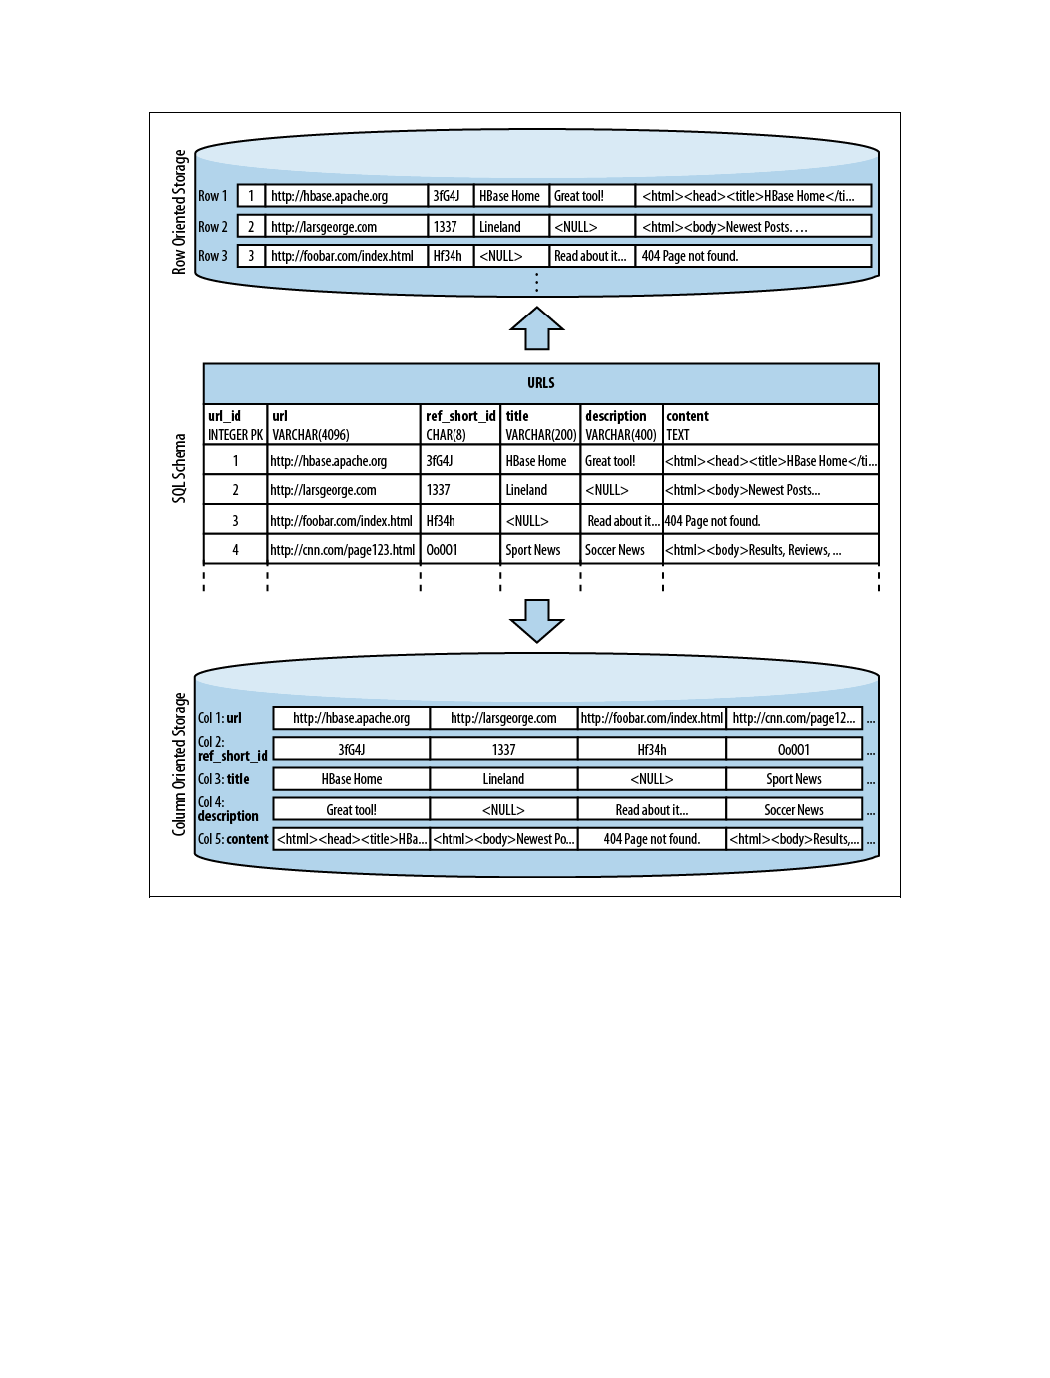
\includegraphics[scale=0.5]{./figures/storage-layout}
    \caption{Example of Storage Layouts}
    \label{fig:storage-layout}
  \end{figure}
}

%%%%%%%%%%%%%%%%%%%%%%%%%%%%%%%%%%%%%%%%%%%%%%%%%%%%%%%%%%
\subsection{The problem with RDBMS}
%%%%%%%%%%%%%%%%%%%%%%%%%%%%%%%%%%%%%%%%%%%%%%%%%%%%%%%%%%
\frame {\frametitle{The Problem with RDBMS}
  \begin{itemize}
  \item \textbf{RDBMS are still relevant}
    \begin{itemize}
    \item Persistence layer for frontend application
    \item Store relational data
    \item Works well for a limited number of records
    \end{itemize}

    \vspace{20pt}

  \item \textbf{Example: Hush}
    \begin{itemize}
    \item Used throughout this course
    \item URL shortener service
    \end{itemize}

    \vspace{20pt}

  \item \textbf{Let's see the ``scalability story'' of such a service}
    \begin{itemize}
    \item Assumption: service must run with a reasonable budget
    \end{itemize}

  \end{itemize}
}

\frame {\frametitle{The Problem with RDBMS}
  \begin{itemize}
  \item \textbf{Few thousands users: use a LAMP stack}
    \begin{itemize}
    \item \textit{Normalize data}
    \item Use foreign keys
    \item Use Indexes
    \end{itemize}

    \begin{figure}[h]
      \centering
      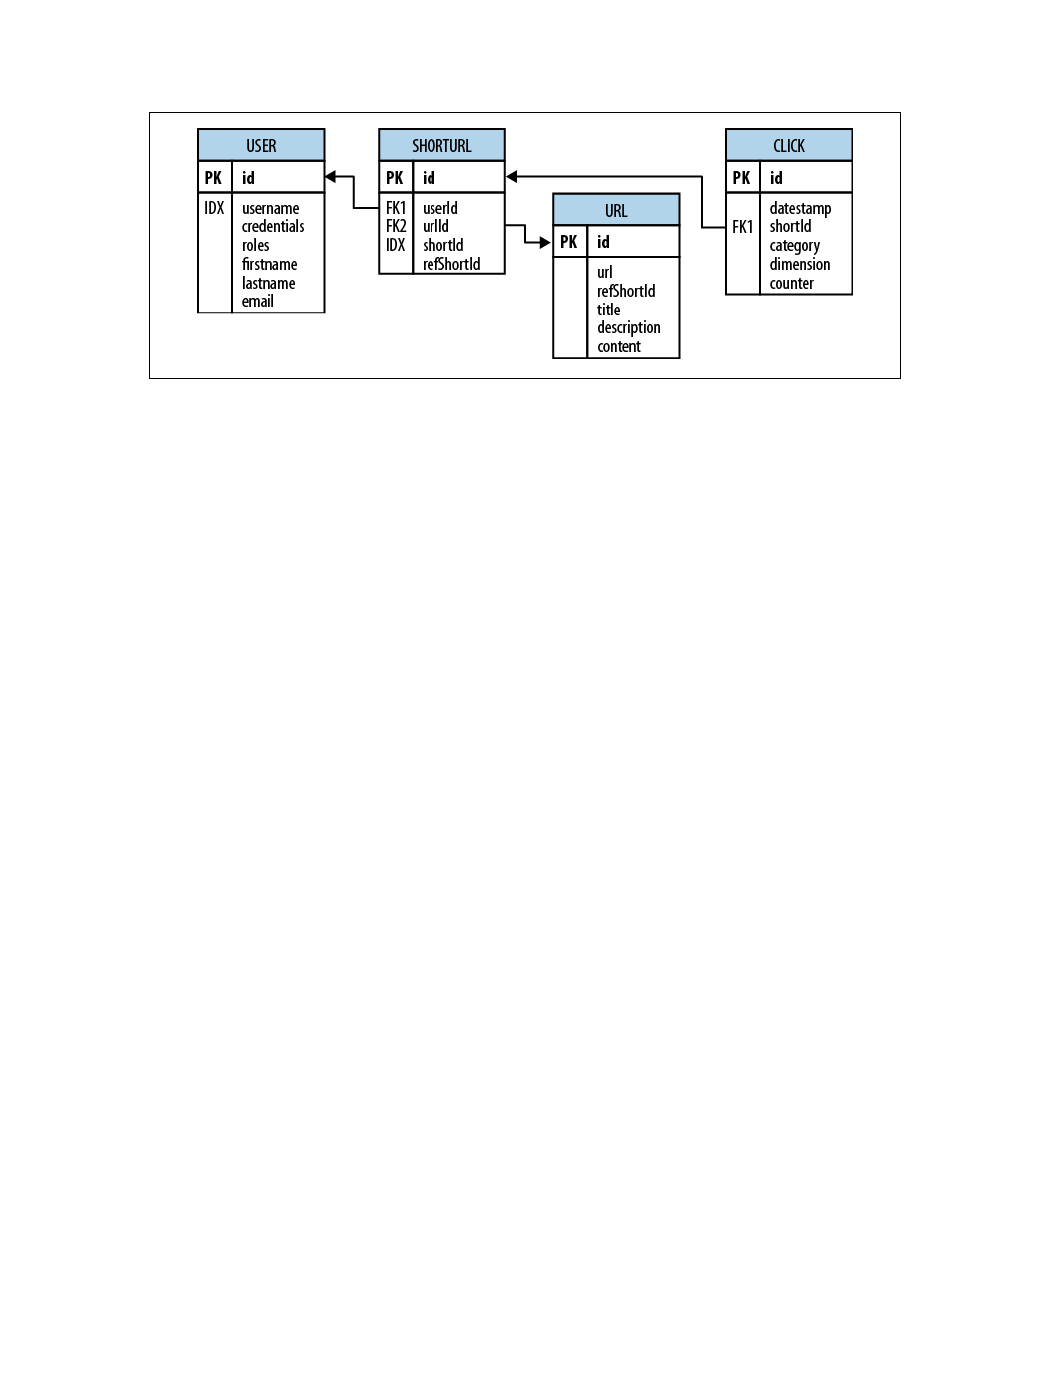
\includegraphics[scale=0.8]{./figures/hush-schema}
      \caption{The Hush Schema expressed as an ERD}
      \label{fig:hush_schema}
    \end{figure}

  \end{itemize}
}

\frame {\frametitle{The Problem with RDBMS}
  \begin{itemize}
  \item \textbf{Find all short URLs for a given user}
    \begin{itemize}
    \item \texttt{JOIN} \texttt{user} and \texttt{shorturl} tables
    \item Use the \texttt{WHERE} clause to select the given user
    \end{itemize}

    \vspace{20pt}

  \item \textbf{Stored Procedures}
    \begin{itemize}
    \item Consistently update data from multiple clients
    \item Underlying DB system guarantees coherency
    \end{itemize}

    \vspace{20pt}

  \item \textbf{Transactions}
    \begin{itemize}
    \item Make sure you can update tables in an \textit{atomic}
      fashion
    \item RDBMS $\to$ \textit{Strong Consistency} (ACID properties)
    \item \textit{Referential Integrity}
    \end{itemize}
  \end{itemize}
}

\frame {\frametitle{The Problem with RDBMS}
  \begin{itemize}
  \item \textbf{Scaling up to tens of thousands of users}
    \begin{itemize}
    \item Increasing pressure on the database server
    \item Adding more application servers is easy: they share their
      state on the same central DB
    \item CPU and I/O start to be a problem on the DB
    \end{itemize}

    \vspace{20pt}

  \item \textbf{Master-Slave architecture}
    \begin{itemize}
    \item Add DB server so that \texttt{READS} can be served in
      parallel
    \item Master DB takes all the writes (which are fewer in the Hush
      application)
    \item Slaves DB replicate Master DB and serve all reads (but you
      need a load balancer)
    \end{itemize}
  
  \end{itemize}
}

\frame {\frametitle{The Problem with RDBMS}
  \begin{itemize}
  \item \textbf{Scaling up to hundreds of thousands}
    \begin{itemize}
    \item \texttt{READS} are still the bottlenecks
    \item Slave servers begin to fall short in serving clients requests
    \end{itemize}

    \vspace{20pt}

  \item \textbf{Caching}
    \begin{itemize}
    \item Add a caching layer, e.g. Memcached or Redis
    \item Offload \texttt{READS} to a fast in-memory system
    \item[$\to$] You lose consistency guarantees
    \item[$\to$] Cache invalidation is critical for having DB and
      Caching layer consistent
    \end{itemize}

  \end{itemize}
}

\frame {\frametitle{The Problem with RDBMS}
  \begin{itemize}
  \item \textbf{Scaling up more}
    \begin{itemize}
    \item \texttt{WRITES} are the bottleneck
    \item The master DB is hit too hard by \texttt{WRITE} load
    \item \textit{Vertical scalability}: beef up your master server
    \item[$\to$] This becomes costly, as you may also have to replace
      your RDBMS
    \end{itemize}

    \vspace{20pt}

  \item \textbf{SQL \texttt{JOINs} becomes a bottleneck}
    \begin{itemize}
    \item Schema de-normalization
    \item Cease using stored procedures, as they become slow and eat
      up a lot of server CPU
    \item Materialized views (they speed up \texttt{READS})
    \item Drop secondary indexes as they slow down \texttt{WRITES}
    \end{itemize}
  \end{itemize}
}

\frame {\frametitle{The Problem with RDBMS}
  \begin{itemize}
  \item \textbf{What if your application needs to further scale up?}
    \begin{itemize}
    \item Vertical scalability vs. Horizontal scalability
    \end{itemize}

    \vspace{20pt}
    
    \item \textbf{Sharding}
      \begin{itemize}
      \item Partition your data across multiple databases
        \begin{itemize}
        \item Essentially you break horizontally your tables and ship
          them to different servers
        \item This is done using fixed boundaries
        \item[$\to$] Re-sharding to achieve load-balancing
        \end{itemize}
      \item[$\to$] This is an operational nightmare
      \item Re-sharding takes a huge toll on I/O resources
      \end{itemize}
  \end{itemize}
}

%%%%%%%%%%%%%%%%%%%%%%%%%%%%%%%%%%%%%%%%%%%%%%%%%%%%%%%%%%
\subsection{NOSQL}
%%%%%%%%%%%%%%%%%%%%%%%%%%%%%%%%%%%%%%%%%%%%%%%%%%%%%%%%%%
\frame {\frametitle{Non-Relational DataBases}
  \begin{itemize}
  \item \textbf{They originally do not support SQL}
    \begin{itemize}
    \item In practice, this is becoming a thin line to make the
      distinction
    \item One difference is in the data model
    \item Another difference is in the consistency model (ACID and
      transactions are generally sacrificed)
    \end{itemize}

    \vspace{20pt}

  \item \textbf{Consistency models and the CAP Theorem}
    \begin{itemize}
    \item Strong: real-time global ordering of operations
    \item Sequential: global ordering of operations that respects 
		client session ordering
	\item Causal: causally related changes are seen in the same
	   	order
    \item Eventual: eventual, steady state replicas convergence
    \item Weak: no guarantee
    \end{itemize}

  \end{itemize}
}

\frame {\frametitle{Dimensions to classify NoSQL DBs}
  \begin{itemize}
  \item \textbf{Data model}
    \begin{itemize}
    \item How the data is stored: key/value, semi-structured,
      column-oriented, ...
    \item How to access data?
    \item Can the schema evolve over time?
    \end{itemize}

    \vspace{20pt}

  \item \textbf{Storage model}
    \begin{itemize}
    \item In-memory or persistent?
    \item How does this affect your access pattern?
    \end{itemize}

    \vspace{20pt}

  \item \textbf{Consistency model}
    \begin{itemize}
    \item Strong or eventual?
    \item This translates in how fast the system handles
      \texttt{READS} and \texttt{WRITES} \cite{Brewer01}
    \end{itemize}
  \end{itemize}
}

\frame {\frametitle{Dimensions to classify NoSQL DBs}
  \begin{itemize}
  \item \textbf{Physical Model}
    \begin{itemize}
    \item Distributed or single machine?
    \item How does the system scale?
    \end{itemize}

    \vspace{20pt}

  \item \textbf{Read/Write performance}
    \begin{itemize}
    \item Top-down approach: understands well the workload!
    \item Some systems are better for \texttt{READS}, other for \texttt{WRITES}
    \end{itemize}

    \vspace{20pt}

  \item \textbf{Secondary indexes}
    \begin{itemize}
    \item Does your workload require them?
    \item Can your system emulate them?
    \end{itemize}
  \end{itemize}
}

\frame {\frametitle{Dimensions to classify NoSQL DBs}
  \begin{itemize}
  \item \textbf{Failure Handling}
    \begin{itemize}
    \item How does each data store handle server failures?
    \item Is it able to continue operating in case of failures?
      \begin{itemize}
      \item This is related to Consistency models and the CAP theorem
      \end{itemize}
      \item Does the system support ``hot-swap''?
    \end{itemize}

    \vspace{20pt}

  \item \textbf{Compression}
    \begin{itemize}
    \item Is the compression method pluggable?
    \item What type of compression?
    \end{itemize}

    \vspace{20pt}

  \item \textbf{Load Balancing}
    \begin{itemize}
    \item Can the storage system seamlessly balance load?
    \end{itemize}
  \end{itemize}
}

\frame {\frametitle{Dimensions to classify NoSQL DBs}
  \begin{itemize}
  \item \textbf{Atomic \texttt{read-modify-write}}
    \begin{itemize}
    \item Easy in a centralized system, difficult in a distributed one
    \item Prevent race conditions in multi-threaded or shared-nothing
      designs
    \item Can reduce client-side complexity
    \end{itemize}

    \vspace{20pt}

  \item \textbf{Locking, waits and deadlocks}
    \begin{itemize}
    \item Support for multiple client accessing data simultaneously
    \item Is locking available?
    \item Is it wait-free, hence deadlock free?
    \end{itemize}

    \vspace{20pt}

    \begin{beamerboxesrounded}{Impedance Match}

        ``One-size-fits-all'' has been long dismissed: need to find
        the perfect match for your problem.

    \end{beamerboxesrounded}

  \end{itemize}
}

%%%%%%%%%%%%%%%%%%%%%%%%%%%%%%%%%%%%%%%%%%%%%%%%%%%%%%%%%%
\subsection{Denormalization}
%%%%%%%%%%%%%%%%%%%%%%%%%%%%%%%%%%%%%%%%%%%%%%%%%%%%%%%%%%
\frame {\frametitle{Database (De-)Normalization}
  \begin{itemize}
  \item \textbf{Schema design at scale}
    \begin{itemize}
    \item A good methodology is to apply the DDI principle \cite{Salmen09}
      \begin{itemize}
      \item Denormalization
      \item Duplication
      \item Intelligent Key design
      \end{itemize}
    \end{itemize}

    \vspace{20pt}

  \item \textbf{Denormalization}
    \begin{itemize}
    \item Duplicate data in more than one table such that at
      \texttt{READ} time no further aggregation is required
    \end{itemize}

    \vspace{20pt}

  \item \textbf{Next: an example based on Hush}
    \begin{itemize}
    \item How to convert a classic relational data model to one that
      fits HBase
    \end{itemize}
  \end{itemize}
}

\frame {\frametitle{Example: Hush - from RDBMS to HBase}
    \begin{figure}[h]
      \centering
      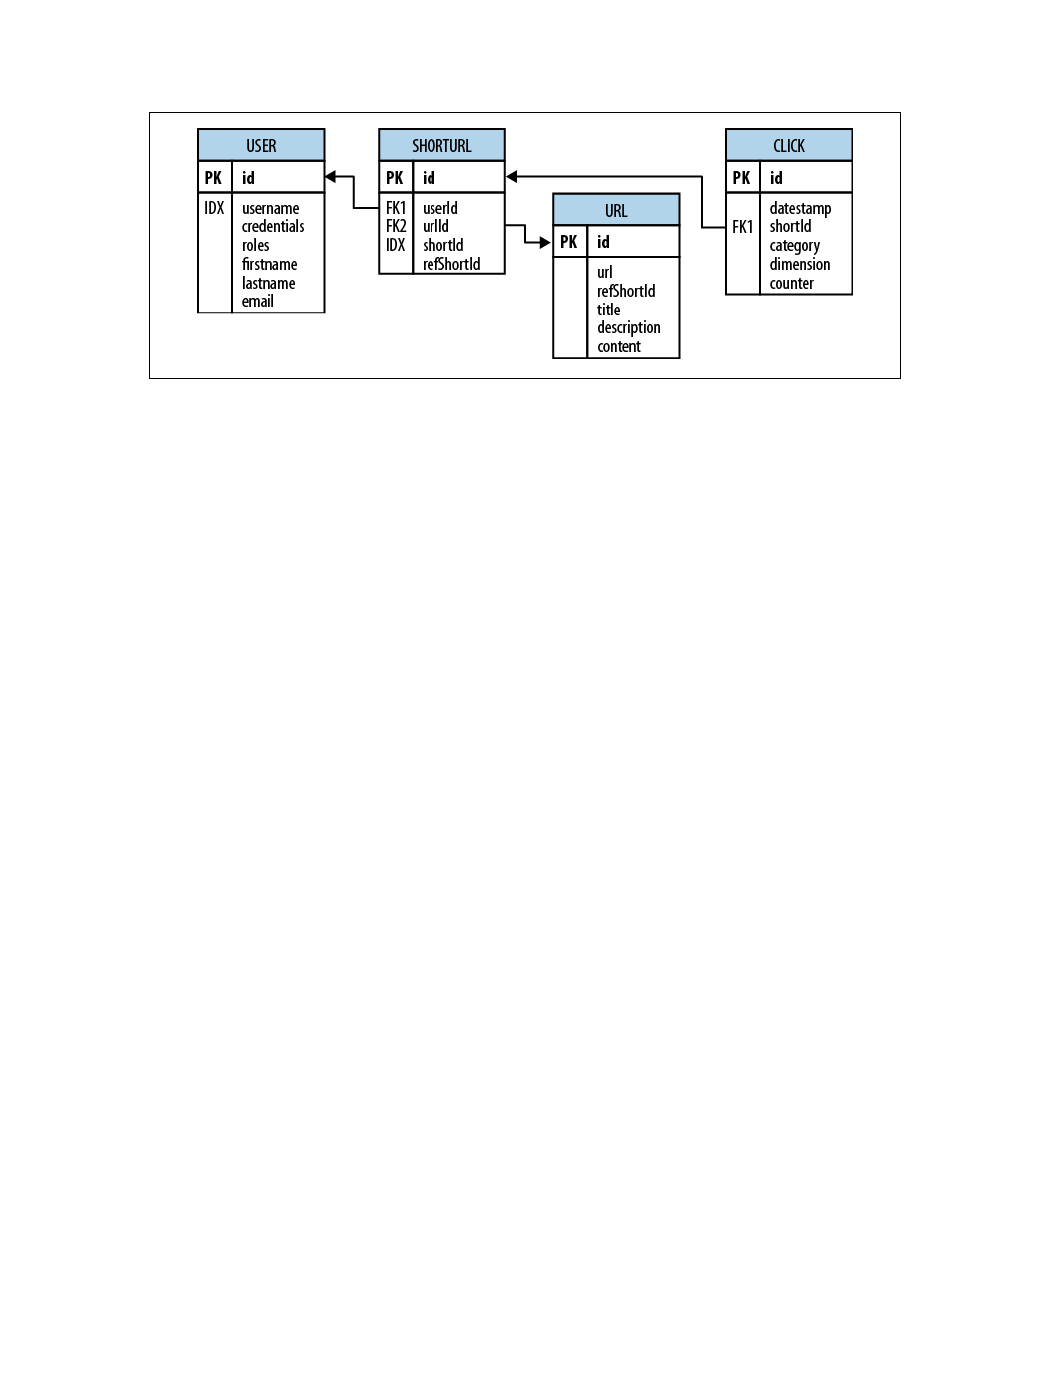
\includegraphics[scale=0.6]{./figures/hush-schema}
      \caption{The Hush Schema expressed as an ERD}
      \label{fig:hush_schema}
    \end{figure}

    \begin{itemize}
    \item \texttt{shorturl} table: contains the short URL
    \item \texttt{click} table: contains click tracking, and other
      statistics, aggregated on a daily basis (essentially, a counter)
    \item \texttt{user} table: contains user information
    \item \texttt{URL} table: contains a replica of the page linked to
      a short URL, including META data and content (this is done for
      batch analysis purposes)
    \end{itemize}
}

\frame {\frametitle{Example: Hush - from RDBMS to HBase}
    \begin{figure}[h]
      \centering
      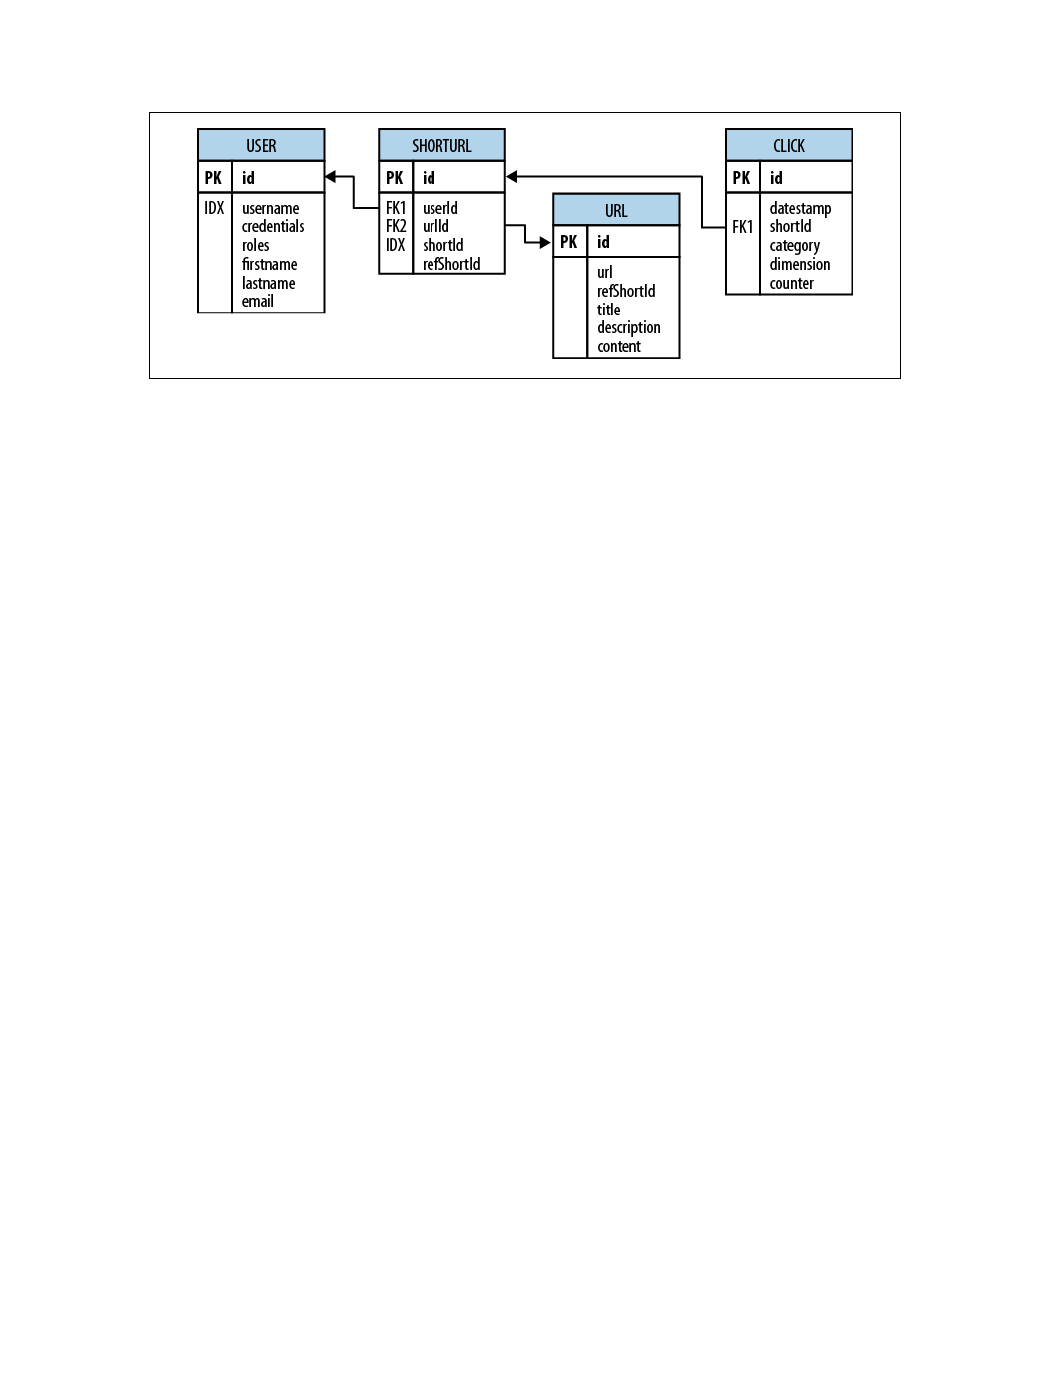
\includegraphics[scale=0.6]{./figures/hush-schema}
      \caption{The Hush Schema expressed as an ERD}
      \label{fig:hush_schema}
    \end{figure}

    \begin{itemize}
    \item \texttt{user} table is indexed on the \texttt{username}
      field, for fast user lookup
    \item \texttt{shorturl} table is indexed on the short URL
      (\texttt{shortId}) field, for fast short URL lookup
   \end{itemize}
}

\frame {\frametitle{Example: Hush - from RDBMS to HBase}
    \begin{figure}[h]
      \centering
      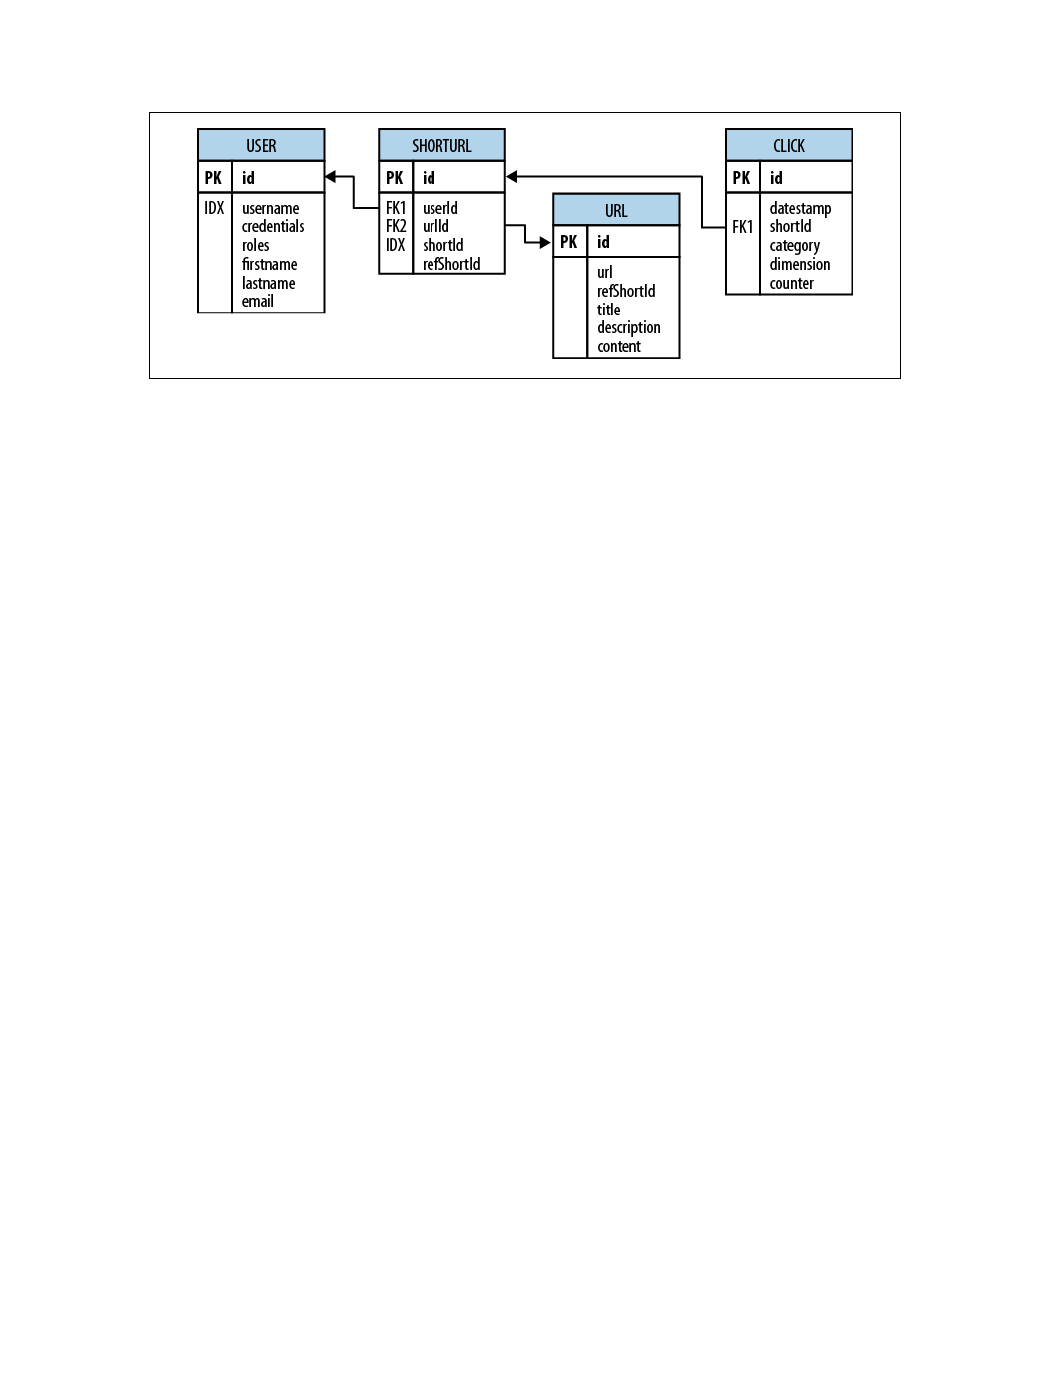
\includegraphics[scale=0.6]{./figures/hush-schema}
      \caption{The Hush Schema expressed as an ERD}
      \label{fig:hush_schema}
    \end{figure}

    \begin{itemize}
    \item \texttt{shorturl} and \texttt{user} tables are related
      through a foreign key relation on the \texttt{userId}
    \item \texttt{URL} table is related to \texttt{shorturl} table
      with a foreign key on the URL id
    \item \texttt{click} table is related to \texttt{shorturl} table
      with a foreign key on the short URL id
    \item NOTE: a web page is stored only once (even if multiple users
      link to it), but each users maintain separate statistics
   \end{itemize}
}

\frame {\frametitle{Example: Hush - from RDBMS to HBase}
  \begin{columns}[c]
    \column{6cm}

    \vspace{-10pt}

    \begin{figure}[h]
      \centering
      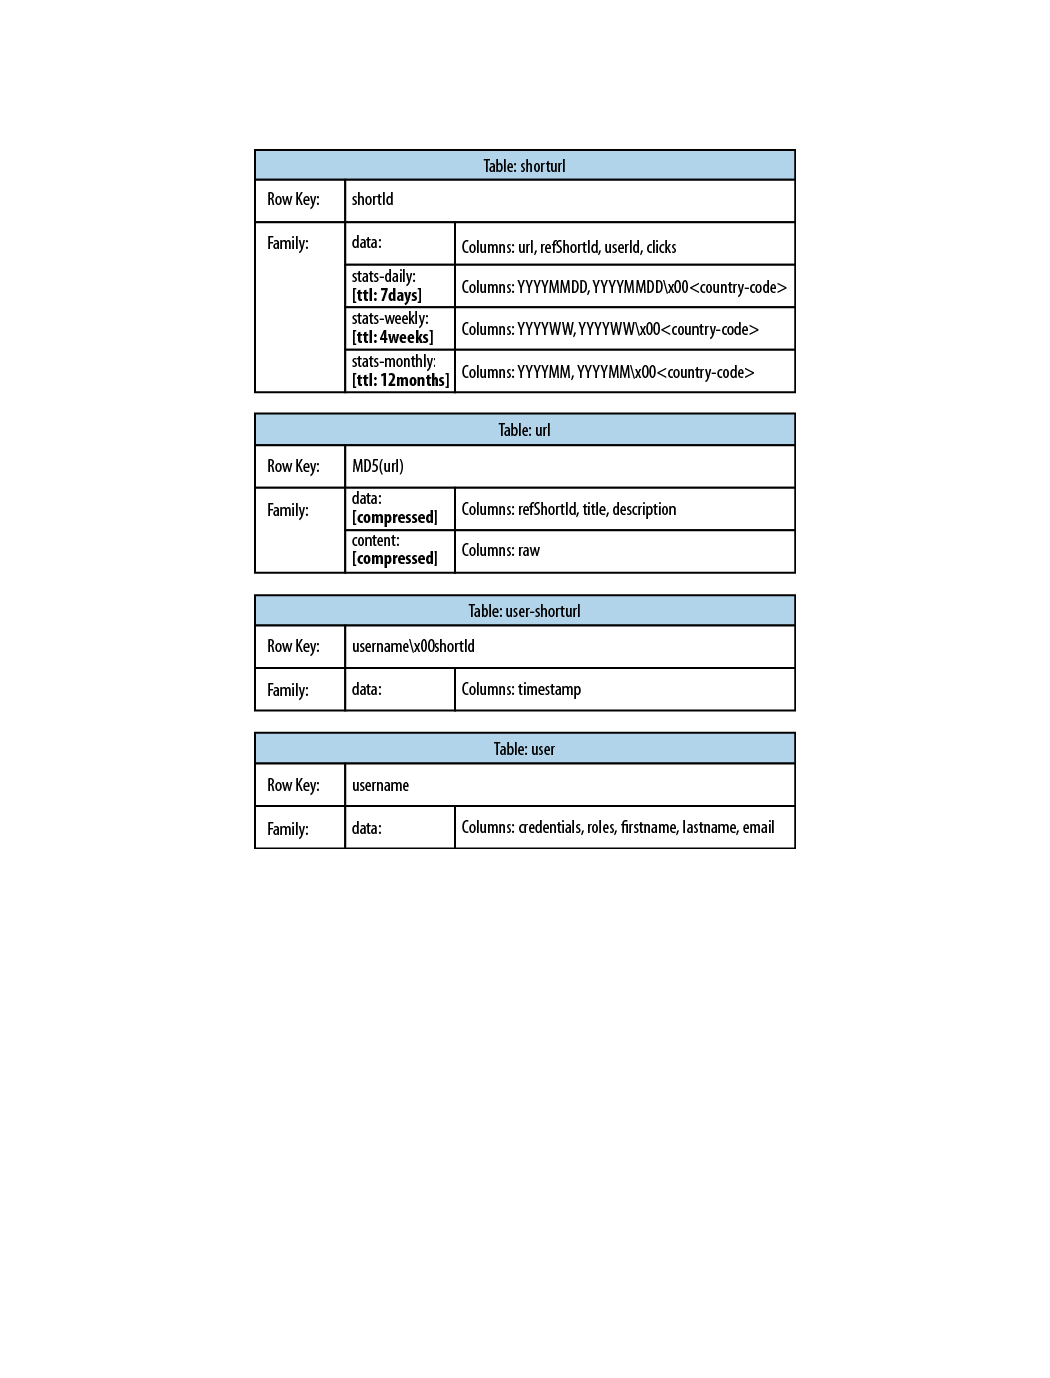
\includegraphics[scale=0.6]{./figures/hush-hbase}
      \caption{The Hush Schema in HBase}
      \label{fig:hush_schema}
    \end{figure}
    
    
    \column{6cm}
    \begin{itemize}
    \item \texttt{shorturl} table: stores each short URL, usage
      statistics (various time-ranges in separate
      \textit{column-families} with distinct \textit{TTL} settings)
      \begin{itemize}
      \item Note the dimensional postfix appended to the time information
      \end{itemize}
      
      \vspace{20pt}
      
    \item \texttt{url} table: stores the downloaded page, and the
      extracted details
      \begin{itemize}
      \item This table uses compression
      \end{itemize}
    \end{itemize}
  \end{columns}
}

\frame {\frametitle{Example: Hush - from RDBMS to HBase}
  \begin{columns}[c]
    \column{6cm}

    \vspace{-10pt}

    \begin{figure}[h]
      \centering
      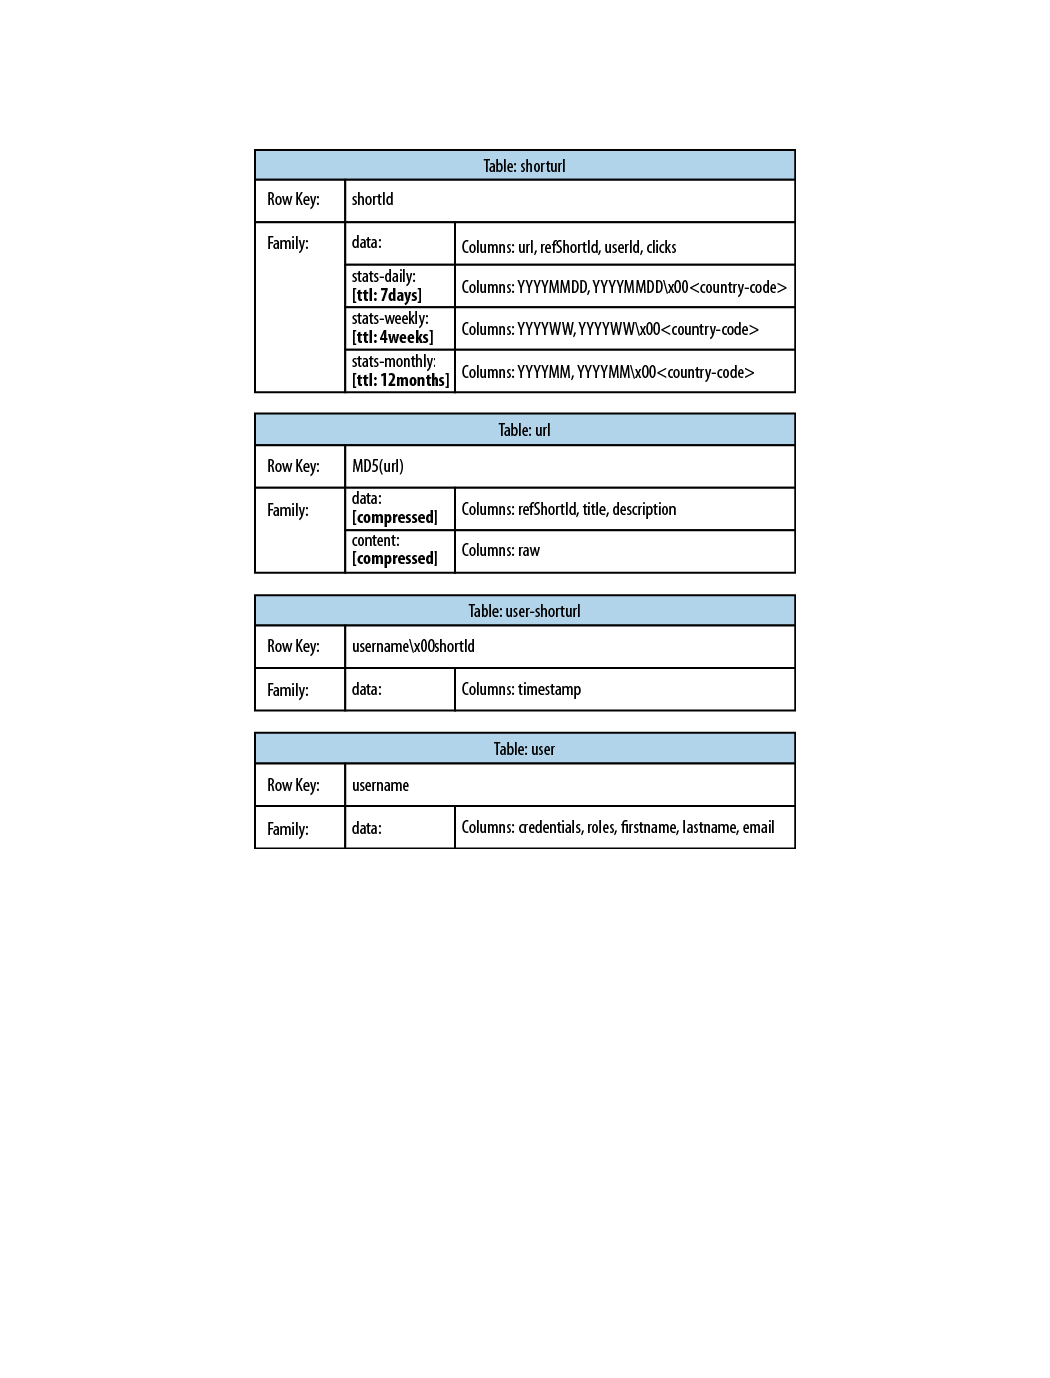
\includegraphics[scale=0.6]{./figures/hush-hbase}
      \caption{The Hush Schema in HBase}
      \label{fig:hush_schema}
    \end{figure}
        
    \column{6cm}
    \begin{itemize}
    \item \texttt{user-shorturl} table: this is a lookup table
      (basically an index) to find all shortIDs for a given user
      \begin{itemize}
      \item Note that this table is filled at \textit{insert time},
        it's not automatically generated by HBase
      \end{itemize}

      \vspace{20pt}

    \item \texttt{user} table: stores user details
    \end{itemize}
  \end{columns}
}

\frame {\frametitle{Example: Hush - RDBMS vs HBase}
  \begin{itemize}
  \item \textbf{Same number of tables}
    \begin{itemize}
    \item Their meaning is different
    \item \texttt{click} table has been absorbed by the
      \texttt{shorturl} table
    \item statistics are stored with the date as the key, so that they
      can be accessed \textit{sequentially}
    \item The \texttt{user-shorturl} table is replacing the foreign
      key relationship, making user-related lookups faster
    \end{itemize}

    \vspace{20pt}

  \item \textbf{Normalized vs. De-normalized data}
    \begin{itemize}
    \item Wide tables and column-oriented design eliminates
      \texttt{JOINs}
    \item \textit{Compound keys} are essential
    \item Data partitioning is based on keys, so a proper
      understanding thereof is essential
    \end{itemize}
  \end{itemize}
}

%%%%%%%%%%%%%%%%%%%%%%%%%%%%%%%%%%%%%%%%%%%%%%%%%%%%%%%%%%
\subsection{HBase Sketch}
%%%%%%%%%%%%%%%%%%%%%%%%%%%%%%%%%%%%%%%%%%%%%%%%%%%%%%%%%%
\frame {\frametitle{HBase building blocks}
  \begin{itemize}
  \item \textbf{The backdrop: BigTable}
    \begin{itemize}
    \item GFS, The Google FileSystem \cite{Ghemawat2003}
    \item Google MapReduce \cite{Dean2004}
    \item BigTable \cite{Chang2006}
    \end{itemize}

    \vspace{20pt}

  \item \textbf{What is BigTable?}
    \begin{itemize}
    \item BigTable is a distributed storage system for managing
      structured data designed to scale to a very large size
    \item BigTable is a sparse, distributed, persistent
      multi-dimensional sorted map
    \end{itemize}
    
    \vspace{20pt}
    
  \item \textbf{What is HBase?}
    \begin{itemize}
    \item Essentially it's an open-source version of BigTable
    \item Differences listed in \cite{George2011}
    \end{itemize}
  \end{itemize}
}

\frame {\frametitle{HBase building blocks}
  \begin{beamerboxesrounded}{}
    Tables, Rows, Columns, and Cells
  \end{beamerboxesrounded}

  \begin{itemize}
  \item \textbf{The most basic unit in HBase is a \textit{column}}
    \begin{itemize}
    \item Each column may have multiple versions, with each distinct
      value contained in a separate \textit{cell}
    \item One or more columns form a \textit{row}, that is addressed uniquely
      by a \textit{row key}
    \end{itemize}

    \vspace{20pt}
    
  \item A table is a collection of rows
    \begin{itemize}
    \item All rows are always \textit{sorted lexicographically} by
      their row key
    \end{itemize}
  \end{itemize}
  \begin{figure}[h]
    \centering
    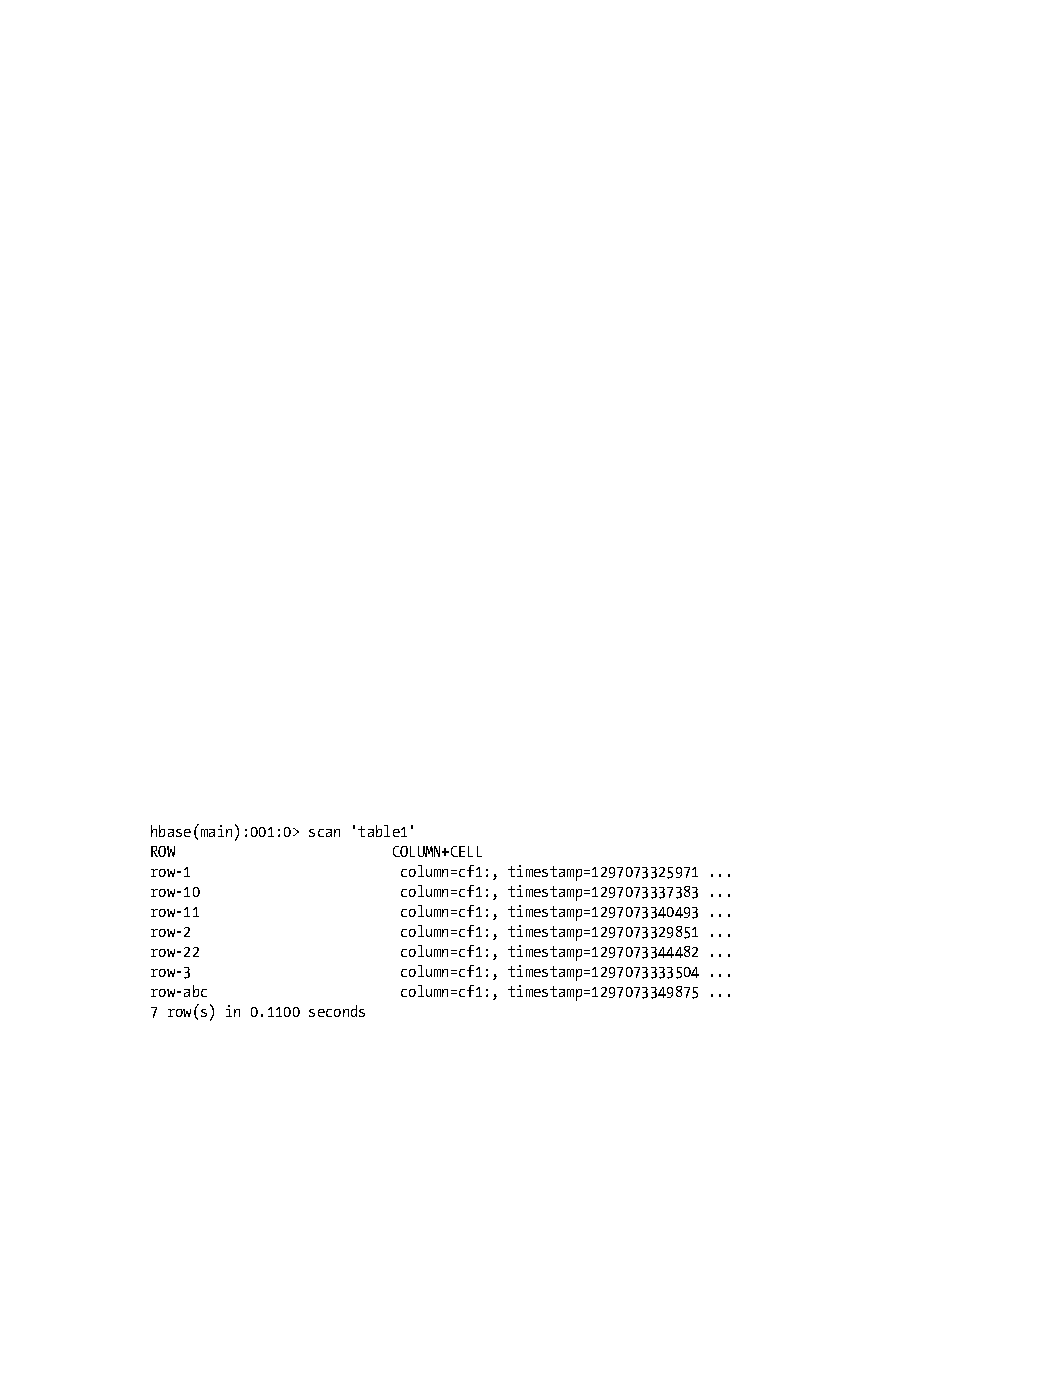
\includegraphics[scale=0.8]{./figures/lexi-sort}
  \end{figure}

}

\frame {\frametitle{HBase building blocks}
  \begin{beamerboxesrounded}{}
    Tables, Rows, Columns, and Cells
  \end{beamerboxesrounded}

  \begin{itemize}
  \item \textbf{Lexicographical ordering of row keys}
    \begin{itemize}
    \item Keys are compared on a binary level, byte by byte, from left
      to right
    \item This can be thought of as a primary index on the row key!
    \item Row keys are \textit{always unique}
    \item Row keys can be any \textit{arbitrary array of bytes}
    \end{itemize}

    \vspace{20pt}

  \item \textbf{Columns}
    \begin{itemize}
    \item Rows are composed of columns
    \item Can have millions of columns
    \item Can be compressed or tagged to stay in memory
    \end{itemize}
  \end{itemize}
}

\frame {\frametitle{HBase building blocks}
  \begin{beamerboxesrounded}{}
    Tables, Rows, Columns, and Cells
  \end{beamerboxesrounded}

  \begin{itemize}
  \item \textbf{Column Families}
    \begin{itemize}
    \item Columns are grouped into \textit{column families}
    \item[$\to$] Semantical boundaries between data
    \item Column families and columns stored together in the same
      low-level storage file, called an \textit{HFile}
    \item Defined when table is created
    \item Should not be changed too often
    \item The number of column families should be reasonable
      [{\color{red}WHY?}]
    \item Column family name composed by printable characters
    \end{itemize}

    \vspace{20pt}

  \item \textbf{References to columns}
    \begin{itemize}
    \item Column ``name'' is called \texttt{qualifier}, and can be any
      arbitrary number of bytes
    \item Reference: \texttt{family:qualifier} (also called the {\color{red}column key})
    \end{itemize}

  \end{itemize}

}

\frame {\frametitle{HBase building blocks}
  \begin{beamerboxesrounded}{}
    Tables, Rows, Columns, and Cells
  \end{beamerboxesrounded}

  \begin{itemize}
  \item \textbf{A note on the \texttt{NULL} value}
    \begin{itemize}
    \item In RDBMS \texttt{NULL} cells need to be set and occupy space
    \item In HBase, \texttt{NULL} cells or columns are simply not stored
    \end{itemize}

    \vspace{20pt}

  \item \textbf{A \textit{cell}}
    \begin{itemize}
    \item Every column value, or cell, is timestamped (implicitly or
      explicitly)
      \begin{itemize}
      \item This can be used to save multiple versions of a value that
        changes over time
      \item Versions are stored in decreasing timestamp, most recent first
      \end{itemize}
    \item Cell versions can be constrained by \textit{predicate
        deletions}
      \begin{itemize}
      \item Keep only values from the last week
      \end{itemize}
    \end{itemize}
  \end{itemize}
}

\frame {\frametitle{HBase building blocks}
  \begin{beamerboxesrounded}{}
    Tables, Rows, Columns, and Cells
  \end{beamerboxesrounded}
  \begin{itemize}
  \item \textbf{Access to data}
    \begin{itemize}
    \item \texttt{(Table, RowKey, Family, Column, Timestamp) $\to$
        Value}
    \item \texttt{SortedMap<RowKey, List<SortedMap<Column, List<Value,
        Timestamp$>\,>\,>\,>$}
    \item[]
    \item The first \texttt{SortedMap} is the table, containing a
      \texttt{List} of column families
    \item The families contain another \texttt{SortedMap}, representing columns
      and a \texttt{List} of value, timestamp tuples
    \end{itemize}

    \vspace{20pt}
    
  \item \textbf{A note on consistency:}
    \begin{itemize}
    \item Row data access is \textbf{atomic} and includes any number
      of columns
    \item There is no further guarantee or transactional feature
      spanning multiple rows
    \item[$\to$] HBase is strongly consistent
    \end{itemize}

  \end{itemize}
}

\frame {\frametitle{HBase building blocks}
  \begin{beamerboxesrounded}{}
    Automatic Sharding
  \end{beamerboxesrounded}

  \begin{itemize}
  \item \textbf{Region}
    \begin{itemize}
    \item This is the basic unit of scalability and load balancing
    \item Regions are contiguous ranges of rows ``stored together'' $\to$
      they are the equivalent of \textit{range partitions} in sharded RDBMS
    \item Regions are \textit{dynamically split} by the system when
      they become too large
    \item Regions can also be merged to reduce the number of storage files
    \end{itemize}
    
    \vspace{20pt}

  \item \textbf{Regions in practice}
    \begin{itemize}
    \item Initially, there is one region
    \item System monitors region size: if a threshold is attained,
      \texttt{SPLIT}
      \begin{itemize}
      \item Regions are split in two at the \textit{middle key}
      \item This creates roughly two equivalent (in size) regions
      \end{itemize}
    \end{itemize}
  \end{itemize}
}

\frame {\frametitle{HBase building blocks}
  \begin{beamerboxesrounded}{}
    Automatic Sharding
  \end{beamerboxesrounded}
  
  \begin{itemize}
  \item \textbf{Region Servers}
    \begin{itemize}
    \item Each region is served by \textit{exactly one Region Server}
    \item Region servers can serve multiple regions
    \item The number of region servers and their sizes depend on the
      capability of a single region server
    \end{itemize}
    
    \vspace{20pt}
    
  \item \textbf{Server failures}
    \begin{itemize}
    \item Regions allow for fast recovery upon failure
    \item Fine-grained Load Balancing is also achieved using regions
      as they can be easily moved across servers
    \end{itemize}
  \end{itemize}
}

\frame {\frametitle{HBase building blocks}
  \begin{beamerboxesrounded}{}
    Storage API
  \end{beamerboxesrounded}
 
  \begin{itemize}
  \item \textbf{No support for SQL}
    \begin{itemize}
    \item CRUD operations using a standard API, available for many
      ``clients''
    \item Data access is not declarative but imperative
    \end{itemize}
    
    \vspace{20pt}
    
  \item \textbf{Scan API}
    \begin{itemize}
    \item Allows for fast iteration over ranges of rows
    \item Allows to limit the number and which column are returned
    \item Allows to control the version number of each cell
    \end{itemize}
    
    \vspace{20pt}
    
  \item \textbf{Read-modify-write API}
    \begin{itemize}
    \item HBase supports single-row transactions
    \item Atomic read-modify-write on data stored in a single row key
    \end{itemize}
  \end{itemize}
}

\frame {\frametitle{HBase building blocks}
  \begin{beamerboxesrounded}{}
    Storage API
  \end{beamerboxesrounded}

  \begin{itemize} 
  \item \textbf{Counters}
    \begin{itemize}
    \item Values can be interpreted as counters and \textbf{updated
        atomically}
    \item Can be read and modified in one operation
    \item[$\to$] Implement global, strongly consistent, sequential counters
    \end{itemize}

    \vspace{20pt}
    
  \item \textbf{Coprocessors}
    \begin{itemize}
    \item These are equivalent to stored-procedures in RDBMS
    \item Allow to push user code in the address space of the server
    \item Access to server local data
    \item Implement lightweight batch jobs, data pre-processing, data summarization
    \end{itemize}
    
  \end{itemize}
}

\frame {\frametitle{HBase building blocks}
  \begin{beamerboxesrounded}{}
    HBase implementation
  \end{beamerboxesrounded}

  \begin{itemize}
  \item \textbf{Data Storage}
    \begin{itemize}
    \item \textit{Store} files are called \texttt{HFiles}
    \item Persistent and ordered \textbf{immutable} maps from key to
      value
    \item Internally implemented as sequences of blocks with an index
      at the end
    \item Index is loaded when the \texttt{HFile} is opened and kept in memory
    \end{itemize}

    \vspace{20pt}

  \item \textbf{Data lookups}
    \begin{itemize}
    \item Since \texttt{HFiles} have a block index, lookup can be done
      with a single disk seek
    \item First, the block possibly containing a given lookup key is
      determined with a \textbf{binary search} in the in-memory index
    \item Then a block read is performed to find the actual key
    \end{itemize}

    \vspace{20pt}

  \item \textbf{Underlying file system}
    \begin{itemize}
    \item Many are supported, usually HBase deployed on top of HDFS
    \end{itemize}

  \end{itemize}
}

\frame {\frametitle{HBase building blocks}
  \begin{beamerboxesrounded}{}
    HBase implementation
  \end{beamerboxesrounded}

  \begin{itemize}
  \item \textbf{\texttt{WRITE} operation}
    \begin{itemize}
    \item First, data is written to a commit log, called WAL
      (write-ahead-log)
    \item Then data is moved into memory, in a structure called
      \texttt{memstore}
    \item When the size of the \texttt{memstore} exceeds a given
      threshold it is flushed to an \texttt{HFile} to disk
    \end{itemize}

    \vspace{20pt}

  \item \textbf{How can HBase write, while serving \texttt{READS} and
      \texttt{WRITES}?}
    \begin{itemize}
    \item Rolling mechanism
      \begin{itemize}
      \item new/empty slots in the \texttt{memstore}
        take the updates
      \item old/full slots are flushed to disk
      \end{itemize}
    \item Note that data in \texttt{memstore} is sorted by keys, matching what
      happens in the \texttt{HFiles}
    \end{itemize}

    \vspace{20pt}

  \item \textbf{Data Locality}
    \begin{itemize}
    \item Achieved by the system looking up for server hostnames
    \item Achieved through intelligent key design
    \end{itemize}
  \end{itemize}
}

\frame {\frametitle{HBase building blocks}
  \begin{beamerboxesrounded}{}
    HBase implementation
  \end{beamerboxesrounded}

  \begin{itemize}
  \item \textbf{Deleting data}
    \begin{itemize}
    \item Since HFiles are immutable, how can we delete data?
    \item A delete marker (also known as \textit{tombstone marker}) is
      written to indicate that a given key is deleted
    \item During the read process, data marked as deleted is skipped
    \item Compactions (see next slides) finalize the deletion process
    \end{itemize}

    \vspace{20pt}

  \item \textbf{\texttt{READ} operation}
    \begin{itemize}
    \item Merge of what is stored in the \texttt{memstores} (data that
      is not on disk) and in the \texttt{HFiles}
    \item The WAL is never used in the \texttt{READ} operation
    \item Several API calls to read, scan data
    \end{itemize}

  \end{itemize}
}

\frame {\frametitle{HBase building blocks}
  \begin{beamerboxesrounded}{}
    HBase implementation
  \end{beamerboxesrounded}
  \begin{itemize}
  \item \textbf{Compactions}
    \begin{itemize}
    \item Flushing data from \texttt{memstores} to disk implies the creation of
      new \texttt{HFiles} each time
    \item[$\to$] We end up with many (possibly small) files
    \item[$\to$] We need to do housekeeping [{\color{red}WHY?}]
    \end{itemize}

    \vspace{20pt}

  \item \textbf{Minor Compaction}
    \begin{itemize}
    \item Rewrites small \texttt{HFiles} into fewer, larger
      \texttt{HFiles}
    \item This is done using an $n$-way merge\footnote{What is MergeSort?}
    \end{itemize}
    \vspace{20pt}

  \item \textbf{Major Compaction}
    \begin{itemize}
    \item Rewrites all files within a column family or a region in a
      new one
    \item Drop deleted data
    \item Perform predicated deletion (e.g. delete old data)
    \end{itemize}
  \end{itemize}
}

\frame {\frametitle{HBase: a glance at the architecture}
  \begin{figure}[h]
    \centering
    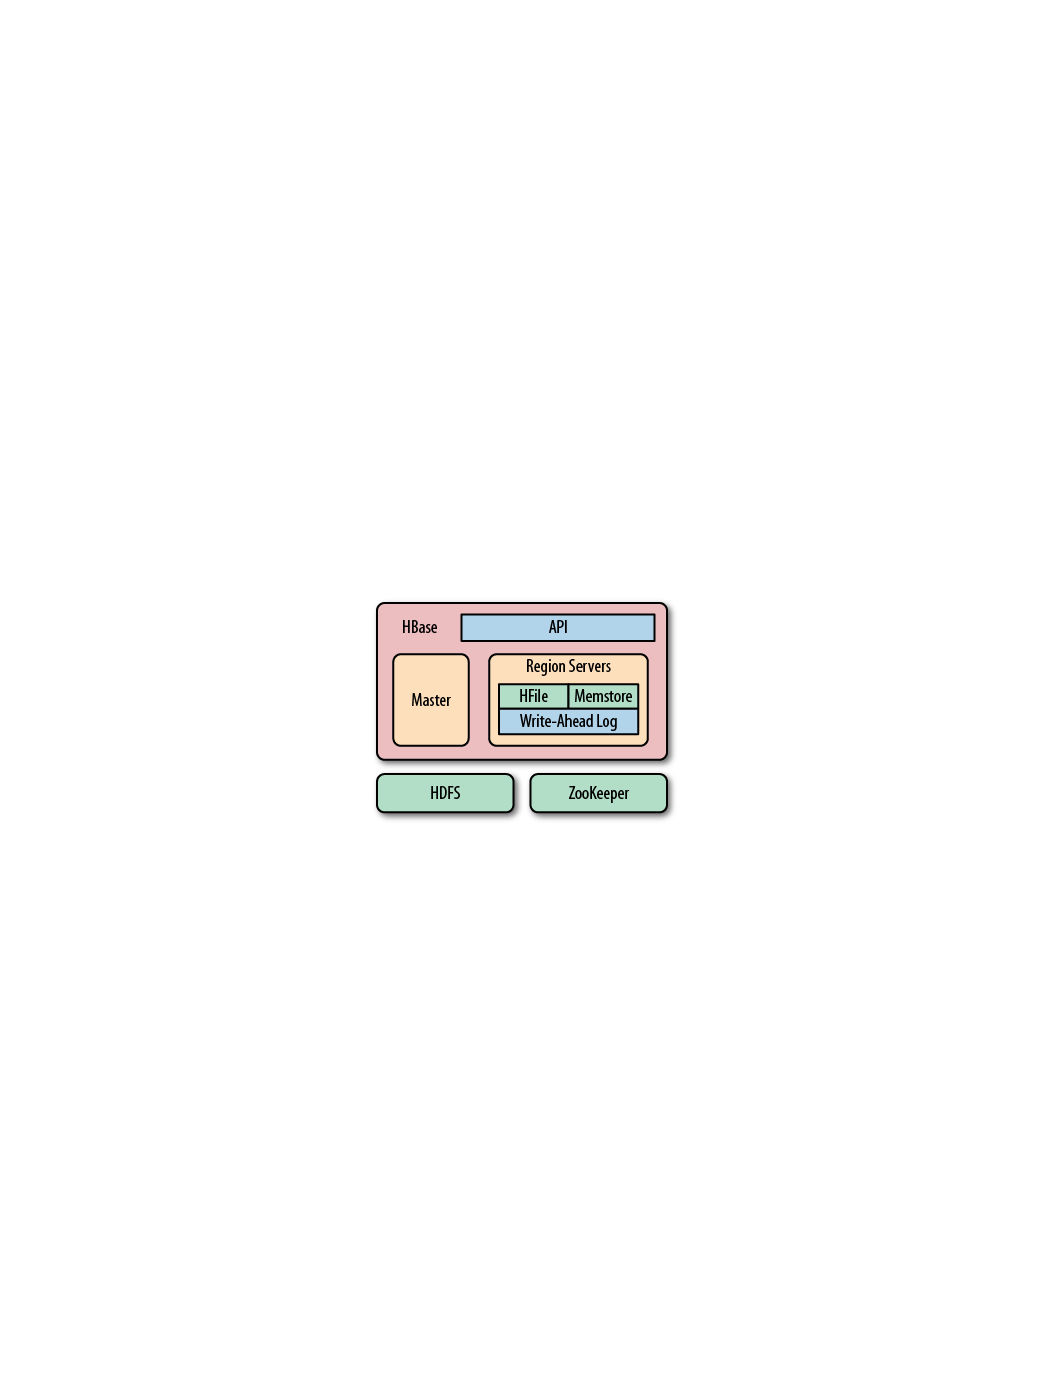
\includegraphics[scale=0.8]{./figures/hbase-arch}
  \end{figure}

  \begin{itemize}
  \item \textbf{Master node: \texttt{HMaster}}
    \begin{itemize}
    \item Assigns regions to region servers using ZooKeeper
    \item Handles load balancing
    \item Not part of the data path
    \item Holds metadata and schema
    \end{itemize}

    \vspace{10pt}

  \item \textbf{Region Servers}
    \begin{itemize}
    \item Handle \texttt{READs} and \texttt{WRITEs}
    \item Handle region splitting
    \end{itemize}
  \end{itemize}
}

